%        File: main.tex
%     Created: 日 10月 27 08:00 下午 2019 C
% Last Change: 日 10月 27 08:00 下午 2019 C
%
\documentclass{ctexart}
\usepackage[a4paper,left=3.2cm,right=3.2cm,top=2.8cm,bottom=2.8cm]{geometry}
\usepackage{fancyhdr}
\usepackage{setspace}
\usepackage{hyperref}
\usepackage{url}
\usepackage{cite}
\usepackage{graphicx}
\usepackage{amsmath}
\usepackage{amssymb}
\usepackage{enumitem}
\usepackage{tikz}
\usepackage{float}
\usepackage{listings}
\usepackage{xcolor}
\usepackage{forest}
\usepackage{pgf}
\usepackage{multirow}
\usepackage{extarrows}
\usetikzlibrary{graphs}
\usetikzlibrary{arrows,automata}
\lstset{language = c,numbers=left, showstringspaces = false, keywordstyle= \color{ blue!70 },commentstyle=\color{red!50!green!50!blue!50}, frame=shadowbox, rulesepcolor= \color{ red!20!green!20!blue!20 } 
} 

\CTEXsetup[format={\Large\bfseries}]{section}
\pagestyle{fancy}

\lhead{中国科学院大学}
\rhead{TextCaps 文献综述}

\cfoot{\thepage}
\usetikzlibrary{graphs}
\renewcommand{\baselinestretch}{1.5}
\title{TextCaps 文献阅读}
\author{\begin{tabular}{ll}
	张佳锋 & $2019/12/14$
\end{tabular}}
\date{}

\begin{document}
\bibliographystyle{IEEEtran}
\maketitle
\zihao{-4}
\CJKfamily{zhsong}
\begin{abstract}
很多小语种想使用深度学习来进行文字识别,然而标注的样本量远远不够用来深度学习。TextCaps主要想解决的问题是减少深度学习的样本量同时不影响识别的精度和模型的泛化能力。在Textcaps文章中,作者使用了3个数据集并同其他模型进行了比较,效果不错。对TextCaps文章进行了细致阅读,对Vinoj Jayasundara的后续研究进行了描述。对本文的参考文献进行了罗列整理。


\textbf{关键字:胶囊网络、小样本学习}
\end{abstract}

\section{Introduction}
手写体字符识别是一个几乎解决了许多主流语言的问题,得益于最近深入学习模型的进展。尽管如此,对于许多其他语言来说,手写体数字识别仍然是一个具有挑战性的问题,因为缺乏足够大的标记数据集来训练深度学习模型。而传统的模型作为线性分类器,K-最近邻分类器、非线性分类器和支持向量机可以被用于这项任务的,但是它们不能实现深度学习模式所提供的接近人类水平的性能。卷积神经网络(CNN)由于具有编码深层特征的能力而取得了最先进的成果。尽管CNN善于理解图像中的低层和高层特性,但这样做,它们在池化层时会丢失有价值的信息。CNN需要大量的训练样本(通常为数千或数万级),以成功训练和分类图像。

TextCaps : Handwritten Character Recognition with Very Small Datasets \cite{jayasundara2019textcaps}是2019年发表在WACV的一篇文章。在这篇文章中,作者提出了一种利用胶囊网络(Capnets)\cite{sabour2017dynamic}解决标记数据集大小小的问题的技术。仅通过利用他们操纵实例化参数\cite{hinton2011transforming}来增强数据的能力。Capnets可以学习图像的属性-在这种情况下是一个字符。这让他们在学习用较少的标记数据来识别字符方面很有用。我们是基于Sabour等人提出的CapsNet架构。\cite{sabour2017dynamic}它包括一个胶囊网络和一个全连接解码网络。我们在对胶囊网络做小改动的同时,用反卷积网络代替了解码器网络。通过在实例化中添加受控制的噪声量,我们对实体进行转换,以描述实际发生的变化。这就产生了一种新的数据生成技术,比仿射变换增强数据更真实。由于重建精度在许多情况下也很重要,我们提出了一种结合损失函数的经验合适的策略。 大大改善了重建效果。我们的系统达到了与世界先进水平相媲美的效果,每类只有200个样本,同时也取得了更好的效果。

本文主要贡献:

1. 在三个数据集上进行了训练并超过了最好的结果,三个数据集分别是EMNIST-letters, EMNIST-balanced 和 EMNIST-digits

2. 在非字符数据集上进行了鲁棒性分析,该数据集是 Fashion-MNIST

3. 每类只用200个样本训练胶囊网络,同时测试样本与之前相当。获得了同样的效果。

4. 分析不同损失函数的效果

注:数据集简介:EMNIST-letters字母数据集共26类、EMNIST-balanced 字母数字数据集共47类、EMNIST-digits数字数据集共10类、Fashion-MNIST时尚单品图像数据集共10类


\section{TextCaps:Origin}
本文主要的点在于胶囊网络字符识别架构和基于实例化参数扰动的图像数据生成技术,下面将分别进行介绍。

\subsection{ 胶囊网络字符识别架构}
胶囊网络结构:

卷积1 :64个3*3核,stride= 2;

卷积2 :128个3*3核,stride= 1;

卷积3 :256个3*3核,stride= 2;

主要胶囊层 :32通道,8维胶囊,每个胶囊包含8个卷积单元,9*9的核并且stride=2;

特征胶囊层:全连接层,每一类是16维胶囊,有多少类别就对应多少个胶囊。

在主胶囊层和特征胶囊层用动态路由算法,采用三次路由迭代。参考自\cite{sabour2017dynamic}

输入胶囊是数据集$J$,28×28的图像。

输出是一个$J\times M \times28$的张量$C$,包含相关的实例化参数。

每一个$C_j,j\in[J]$是第$j^th$的训练样本的实例化参数矩阵
采用独热编码的形式,在将$C$输入到解码网络之前,只有是这个类的才不为零,其他为零。经过这个操作后,记为$\hat{C}$

特征胶囊层是一个全连接层后面跟着五个反卷积层,该层的输入是$\hat{C}$输出为28×28的图像。在特征胶囊层中除了最后一层是采用sigmoid激活函数,其他层用RELU激活函数。

作者在这种情况下做实验发现,采用大量样本才能获得好的结果。这显然是不行的,同时主胶囊层已经很完美了。问题出在特征胶囊层无法很好的重建。其原因还是在于样本数量不够。因此提出了一种新的训练样本生成方法,它利用胶囊网络中实例化参数的概念来增强原始训练样本

\subsection{基于实例化参数扰动的图像数据生成技术}

因为已经可以提取到足够多的特征,所以可以通过这些特征向量来描述任意字符。通过训练好的模型已经可以通过实例化参数来进行很好的重建了。因此,想在实例化参数中加入一些噪声,以此来产生新的样本。

首先采用原始的包含2000个样本的数据集。为了保证一致性,取每一个类别中的前200个。采用这么多的样本训练胶囊网络。训练结果称为$M_{1,caps},M_{1,dec}$,前面表示主胶囊层,后面表示特征胶囊层。再通过这个网络生成一部分样本,生成样本的过程中保留输入到特征胶囊层的实例化参数。


生成的样本不太清晰,为了解决这个问题,对生成样本进行了锐化。将锐化后的生成样本加上前面的原始样本作为新的数据集再去训练,得到$\widetilde{M_{1,dec}}$。训练这个网络的目的在于为了消除模糊。结束后对这次生成的结果进行挑选。因为会产生一些不符合实际的样本。

最后将这个新的网络$\widetilde{M_{1,dec}}$和之前保留的实例化参数结合,通过对实例化参数中的各个参数进行扰动来生成新的样本。

在对实例化参数进行扰动的时候,作者通过分析选择了对结果影响较大的前两个参数进行扰动。为了使得结果可控,每次只扰动一个参数。每扰动一次,对于每一类生成50个新的随机的样本。对于扰动的幅度作者进行了限制以避免出现无效的图像。


通过这样的方法增加样本量之后,重新训练识别网络,并获得很好的效果。









\subsection{不同的重建损失函数}
作者在此节提出了4种损失函数,分别是MSE,L1 Norm, SSIM,Binary Cross-Entropy (BCE)。并且采用了两两结合的方法。具体来说就是每次生成图像的时候采用两个损失函数生成两张图片,对每张图片的各个像素点与原图进行对比,选择靠近真实点的像素点作为真正的输出。
\subsection{实验结果}
实验结果具体看Table2截图
\begin{figure}[!htbp]
	\centering
	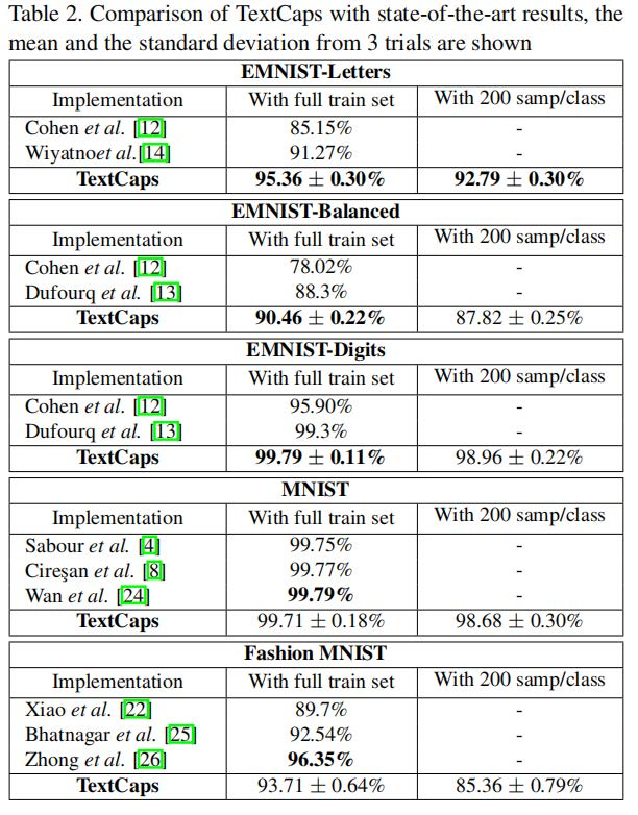
\includegraphics[scale = 1]{Fig/results.pdf}
	\caption{实验结果与对比图}
	\label{fig:results}
\end{figure}








\section{Follow Research}
\subsection{DeepCaps: Going Deeper with Capsule Networks}
本文摘要翻译\cite{rajasegaran2019deepcaps}
胶囊网络在深度学习中是一个很有前途的概念,目前他在几个关键的数据集上的的表现低于标准结果,其真正的潜力还没有得到充分的发挥。深度卷积神经网络的成功给我们带来了启示,我们介绍DeepCaps,顾名思义它是一个深度胶囊网络。它基于最新的三维卷积算法。 使用DeepCaps,我们在CIFAR10,SVHN和Fashion MNIST的胶囊网络领域中超越了最新技术成果,同时使参数数量减少了68%。

此外,我们提出了一个与类无关的解码器网络,该网络加强了重建损失作为正则化项的使用。 这导致了解码器的有趣特性,它使我们能够识别和控制由实例化参数表示的图像的物理属性。

本文核心:提出了DeepCaps网络,该网络对于数据集CIFAR10, SVHN和 Fashion MNIST的结果超过了以往的胶囊网络识别结果。

\subsection{TreeCaps: Tree-Structured Capsule Networks for Program Source Code Processing}
本文摘要翻译\cite{jayasundara2019treecaps}:程序理解是软件开发和维护过程中的一项基本任务。软件开发人员通常需要先了解大量现有代码,然后才能开发新功能或修复现有程序中的错误。能够自动处理编程语言代码并准确提供代码功能摘要可以极大地帮助开发人员减少花在代码导航和理解上的时间,从而提高生产率。与自然语言文章不同,编程语言中的源代码通常遵循严格的语法结构,并且通过复杂的控制流和数据流,彼此远离的代码元素之间可能存在依赖关系。对基于树的卷积神经网络(TBCNN)和门控图神经网络(GGNN)的现有研究无法准确地捕获代码元素之间的基本语义依赖性。在本文中,我们提出了新颖的基于树的胶囊网络(TreeCaps)和以自动方式处理程序代码的相关技术,该方法对代码的语法结构进行编码并更准确地捕获代码依赖性。基于对用不同编程语言编写的程序的评估,我们表明,在对许多程序的功能进行分类时,基于TreeCaps的方法可以胜过其他方法。

本文核心:基于胶囊网络的程序理解以及处理

\section{Introduction of Main References}

对于本篇论文的思想,主要引用自原文的[4][5]两篇参考文献。
这是两篇大作,因此只给出了一些网址以供参考。

\subsection{ Dynamic routing between capsules[4]}
本篇文章\cite{sabour2017dynamic}由谷歌学术统计被引用1112次。

对于这篇文章的讲解,可以参考网站
\href{https://www.zhihu.com/question/67287444?sort=created}{知乎}

翻译\href{https://www.jianshu.com/p/8d4eefae0444}{简书翻译}

\subsection{Transforming auto-encoders[5]}
本文章\cite{hinton2011transforming}由谷歌学术统计被引用535次。
本文翻译\href{https://blog.csdn.net/XinyanH/article/details/78735573}{CSDN翻译}



%reference
\newpage
\bibliography{./Bib/ref}
\end{document}


